\documentclass{beamer}
\usetheme{Boadilla}
\usepackage{pgfplots}
\usepackage{tikz}
\usetikzlibrary{shapes,arrows,chains}
\usetikzlibrary[calc]
\usepackage{amssymb,amsmath,mathrsfs,stmaryrd,bm,amsthm,amsfonts}
\usepackage{pgfplotstable}
\usepackage{biblatex}
\addbibresource{../paper/biblio.bib}
\renewcommand{\footnotesize}{\scriptsize}
\usepackage{pifont}
\usetikzlibrary{math}

\newcommand{\tikzxmark}{
\tikz[scale=0.25] {
    \draw[line width=0.7,color=red,line cap=round] (0,0) to [bend left=6] (1,1);
    \draw[line width=0.7,color=red,line cap=round] (0.2,0.95) to [bend right=3] (0.8,0.05);
}}
\newcommand{\tikzcmark}{
\tikz[scale=0.25] {
    \draw[line width=0.7,color=green,line cap=round] (0.25,0) to [bend left=10] (1,1);
    \draw[line width=0.8,color=green,line cap=round] (0,0.35) to [bend right=1] (0.23,0);
}}

%Information to be included in the title page:
\title[Shapley compositions]{Explaining probabilistic predictions on the simplex\\with Shapley compositions}
\author[Paul-Gauthier Noé]{\textbf{Paul-Gauthier Noé} \inst{1}, Miquel Perelló-Nieto \inst{2},\\Peter Flach \inst{2}, Jean-François Bonastre \inst{1}}
\institute[]{\inst{1} Avignon Université \and \inst{2} University of Bristol}

\date[LIA seminar]
{LIA seminar, Avignon Université\\January 18, 2024}
\begin{document}

\frame{\titlepage}

\section{Introduction}

\begin{frame}
\frametitle{Introduction}

\textbf{Local explanation in machine learning:}

\begin{figure}
  \centering
  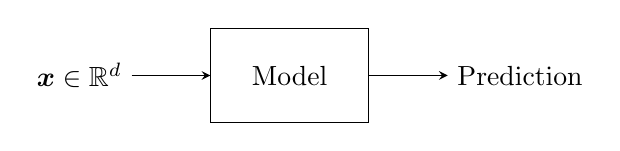
\begin{tikzpicture}
  \node [draw,
	minimum width=2cm,
	minimum height=1.2cm
        ]  (model) {Model};
        \node [left=1cm of model] (x) {$\bm{x}\in\mathbb{R}^d$};
        \node [right=1cm of model] (pred) {Prediction};
        \draw[-stealth] (x.east) -- (model.west);
        \draw[-stealth] (model.east) -- (pred.west);
      \end{tikzpicture}
    \end{figure}
    \textit{Given one instance $\bm{x}$ with $d$ features, what is the contribution/effect of a feature's value on the prediction?}
    

    \begin{center}
      $\neq$ Global explanation
    \end{center}
  \end{frame}

  \begin{frame}
    \frametitle{Introduction}
    Examples of local explanation methods:
    \begin{itemize}
    \item Local Interpretable Model-Agnostic Explanations (LIME) \footfullcite{ribeiro2016should},
    \item Shapley values \footfullcite{vstrumbelj2014explaining} (SHAP toolkit \footfullcite{NIPS2017_7062})
      
    \end{itemize}
  \end{frame}

  \begin{frame}
    \frametitle{Introduction}
    \textbf{Shapley values in cooperatibe game theory}\footfullcite{shapley1953value}
    \begin{itemize}
    \item Distributes the total payoff among the players.
    \item The unique quantity respecting a set of desired axiomatic properties:
      \begin{itemize}
      \item Linearity:\\
        \begin{equation}
          \phi_{\alpha v + (1-\alpha)w}(i) = \alpha \phi_{v}(i) + (1-\alpha) \phi_{w}(i),
        \end{equation}
        for a player $i$ and two games $v$ and $w$, and for $\alpha \in [0,1]$
      \item Efficiency,
        \begin{equation}
          \sum_{i\in\mathcal{C}} \phi_{v}(i) = v (\mathcal{C}),
        \end{equation}
        (the sum of the value is equal to the total payoff)
      \item Symmetry
      \end{itemize}
    \end{itemize}
  \end{frame}

  \begin{frame}
    \frametitle{Introduction}
    \textbf{Shapley values in machine learning}
    \begin{itemize}
    \pause
    \item Features are treated as players, and the scalar output of the model as the payoff,
    \begin{figure}
  \centering
  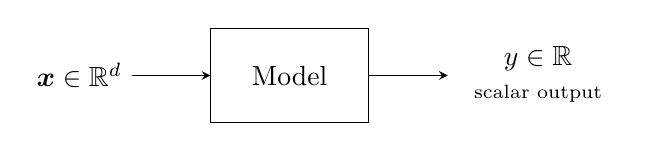
\begin{tikzpicture}
  \node [draw,
	minimum width=2cm,
	minimum height=1.2cm
        ]  (model) {Model};
        \node [left=1cm of model] (x) {$\bm{x}\in\mathbb{R}^d$};
        \node [right=1cm of model] (pred) {\begin{tabular}{c}$y\in\mathbb{R}$\\\scriptsize scalar output\end{tabular}};
        \draw[-stealth] (x.east) -- (model.west);
        \draw[-stealth] (model.east) -- (pred.west);
      \end{tikzpicture}
    \end{figure}
    \pause
    \item Binary classifier, regressor with one-dimensional output \tikzcmark
    \pause
    \item Multiclass classifier \tikzxmark

          ex: The output of a softmax layer lives on a multidimensional simplex!
        \end{itemize}

  \end{frame}


  \begin{frame}
    \frametitle{Introduction}

\tikzset{%
  every neuron/.style={
    circle,
    draw,
    minimum size=0.5cm
  },
  neuron missing/.style={
    draw=none, 
    scale=2,
    text height=0.333cm,
    execute at begin node=\color{black}$\vdots$
  },
}
    
\begin{figure}
  \centering
  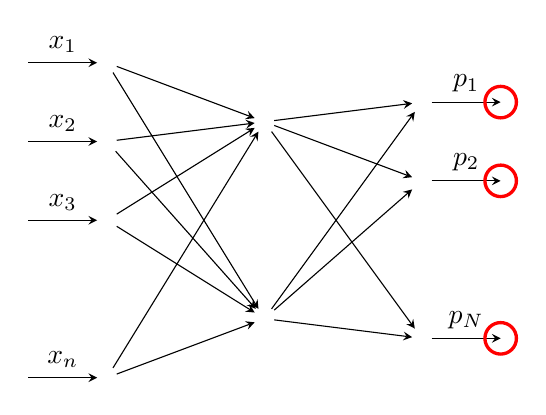
\begin{tikzpicture}[>=stealth]

\foreach \m/\l [count=\y] in {1,2,3,missing,4}
  \node [every neuron/.try, neuron \m/.try] (input-\m) at (0,2.5-\y) {};

\foreach \m [count=\y] in {1,missing,2}
  \node [every neuron/.try, neuron \m/.try ] (hidden-\m) at (2,2-\y*1.25) {};

\foreach \m [count=\y] in {1,2,missing,3}
  \node [every neuron/.try, neuron \m/.try ] (output-\m) at (4,2-\y) {};

\foreach \l [count=\i] in {1,2,3,n}
  \draw [<-] (input-\i) -- ++(-1,0)
    node [above, midway] {$x_\l$};

\foreach \l [count=\i] in {1,n}
  \node [above] at (hidden-\i.north) {};

\foreach \l [count=\i] in {1,2,N}
  \draw [->] (output-\i) -- ++(1,0)
  node [above, midway] {$p_\l$};

\foreach \l [count=\i] in {1,2,N}
  \draw [very thick, color=red] (output-\i)+(1,0) circle (0.2);

\foreach \i in {1,...,4}
  \foreach \j in {1,...,2}
    \draw [->] (input-\i) -- (hidden-\j);

\foreach \i in {1,...,2}
  \foreach \j in {1,...,3}
    \draw [->] (hidden-\i) -- (output-\j);

  \end{tikzpicture}
\end{figure}
\begin{center}
  Some explain the output one-by-one,
\end{center}
\pause

        \begin{center}
          But a probability distribution lives on a simplex,\\
          \textbf{The relative information matter!!}
        \end{center}
        
      \end{frame}

  \begin{frame}
    \frametitle{Introduction}

\tikzset{%
  every neuron/.style={
    circle,
    draw,
    minimum size=0.5cm
  },
  neuron missing/.style={
    draw=none, 
    scale=2,
    text height=0.333cm,
    execute at begin node=\color{black}$\vdots$
  },
}
    
\begin{figure}
  \centering
  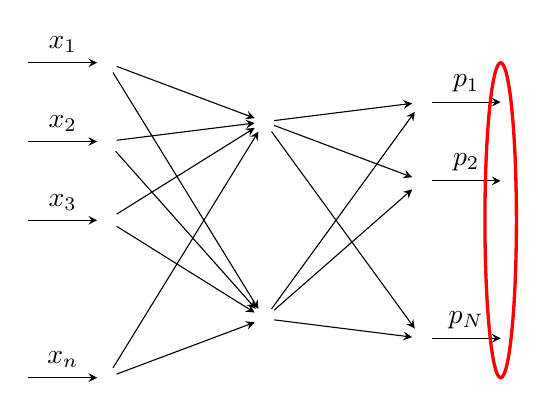
\begin{tikzpicture}[>=stealth]

\foreach \m/\l [count=\y] in {1,2,3,missing,4}
  \node [every neuron/.try, neuron \m/.try] (input-\m) at (0,2.5-\y) {};

\foreach \m [count=\y] in {1,missing,2}
  \node [every neuron/.try, neuron \m/.try ] (hidden-\m) at (2,2-\y*1.25) {};

\foreach \m [count=\y] in {1,2,missing,3}
  \node [every neuron/.try, neuron \m/.try ] (output-\m) at (4,2-\y) {};

\foreach \l [count=\i] in {1,2,3,n}
  \draw [<-] (input-\i) -- ++(-1,0)
    node [above, midway] {$x_\l$};

\foreach \l [count=\i] in {1,n}
  \node [above] at (hidden-\i.north) {};

\foreach \l [count=\i] in {1,2,N}
  \draw [->] (output-\i) -- ++(1,0)
  node [above, midway] {$p_\l$};

\foreach \i in {1,...,4}
  \foreach \j in {1,...,2}
    \draw [->] (input-\i) -- (hidden-\j);

\foreach \i in {1,...,2}
  \foreach \j in {1,...,3}
    \draw [->] (hidden-\i) -- (output-\j);

  \draw [very thick, color=red] (5,-0.5) ellipse (0.2 and 2);
    
  \end{tikzpicture}
\end{figure}
        \begin{center}
          We will explain the probablities all together using the\\
          \emph{Aitchison geometry of the simplex}\footfullcite{aitchison1982,pawlowskymodeling}.
        \end{center}
        
  \end{frame}


  \begin{frame}{Outline}
    \tableofcontents
  \end{frame}
  
\section{The Shapley values in machine learning}


\begin{frame}
\frametitle{The Shapley values in machine learning}

We want to explain a prediction $f(\bm{x})$ on the instance $\bm{x}\in\mathcal{X}\subset\mathbb{R}^d$, where $f:\mathcal{X}\to\mathbb{R}$ is the learned model.
\begin{figure}
  \centering
  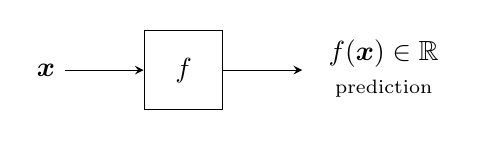
\begin{tikzpicture}
  \node [draw,
	minimum width=1cm,
	minimum height=1cm
        ]  (model) {$f$};
        \node [left=1cm of model] (x) {$\bm{x}$};
        \node [right=1cm of model] (pred) {\begin{tabular}{c}$f(\bm{x})\in\mathbb{R}$\\\scriptsize prediction\end{tabular}};
        \draw[-stealth] (x.east) -- (model.west);
        \draw[-stealth] (model.east) -- (pred.west);
      \end{tikzpicture}
    \end{figure}

\pause
Some notation. Let:
\begin{itemize}
\item $\text{Pr}$ be the probability distribution over $\mathcal{X}$ of the data.
\pause
\item $S\subseteq \mathcal{I}=\{1,2,\dots d\}$ be a subset of indices,
\pause
\item $\bm{x}_S$ refers to an instance $\bm{x}$ restricted to the features indicated by the indices in $S$.
\end{itemize}

\end{frame}

\begin{frame}
  \frametitle{The Shapley values in machine learning}
The \textbf{value function}:
\begin{equation}
  \begin{aligned}
    v_{f,\bm{x},\text{Pr}}: 2^{\mathcal{I}} &\to \mathbb{R},\\
    S &\mapsto \mathbb{E}_\text{Pr}[f(\bm{x})\mid \bm{x}_S],
  \end{aligned}
\end{equation}
where $\mathbb{E}_{\text{Pr}}[f(\bm{x}) \mid \bm{x}_S] = \int_{\bm{x} \in \mathcal{X}}f(\bm{x})\text{Pr}(\bm{x} \mid \bm{x}_S)d\bm{x}$.
\vspace{1cm}

When an instance $\bm{x}$ is observed, the expected value of the prediction is simply $\mathbb{E}[f(\bm{x}) \mid \bm{x}] = f(\bm{x})$. However, when only $\bm{x}_S$ is given with $\mathcal{S} \neq \mathcal{I}$, there is uncertainty about the non-observed features and we therefore compute the expected prediction given $\bm{x}_S$.
\end{frame}

\begin{frame}
\frametitle{The Shapley values in machine learning}
  
The \textbf{contribution} of the feature indexed by $i \notin S$ in the prediction $f(\bm{x})$ given the known features indexed by $S$ is given by:
\begin{equation}
  \label{eq:contrib}
  c_{f,\bm{x},\text{Pr}}(i,\bm{X}_S) = v_{f,\bm{x},\text{Pr}}(\bm{X}_{S\cup\{i\}}) - v_{f,\bm{x},\text{Pr}}(\bm{X}_S),
\end{equation}

This measures the contribution of the $i$th features with a particular \emph{coalition} of features indexed by $S$.
\end{frame}

\begin{frame}
  \frametitle{The Shapley values in machine learning}
  
 The whole contribution of the $i$th feature is computed by averaging this quantity over all possible coalitions of features as follows:
\begin{equation}
  \phi_{f,\bm{x},\text{Pr}}(i) = \frac{1}{d!} \sum_{\pi}c_{f,\bm{x},\text{Pr}}(i,\pi^{<i}_{\bm{X}}),
\end{equation}
where $\pi$ is a permutation of the set $\mathcal{I}$ of indexes and $\pi^{<i}_{\bm{X}}$ is the features of $\bm{X}$ coming before the $i$th feature in the ordering given by $\pi$.
\pause
\begin{center}
  This quantity is known as the {\Large\textbf{Shapley value}} for the $i$th feature.
\end{center}

\end{frame}

\begin{frame}
  \frametitle{The Shapley values in machine learning}
  
  It comes from cooperative game theory and is known to be the only quantity respecting a set of desired axiomatic properties \footfullcite{shapley1953value}.
  \begin{itemize}
    \pause
\item Linearity with respect to the model ($\alpha, \beta \in \mathbb{R}$): $\phi_{\alpha f +\beta g}(i) = \alpha \phi_f(i) + \beta \phi_g(i)$,
    \pause
\item The ``centered'' learned model is additively separable with respect to the Shapley values:
\begin{equation}
  f(\bm{x})-\mathbb{E}_{\text{Pr}}[f(\bm{X})] = \sum_{i=1}^{d} \phi_f(i),
\end{equation}
which is known as the \emph{efficiency} property.
    \pause
\item Symmetry
\end{itemize}

\end{frame}

\begin{frame}
  \frametitle{The Shapley values in machine learning}
  Example of explanation:
  \begin{figure}
    \centering
    \includegraphics[width=\linewidth]{figures/example_from_shap}
    \caption{Explanation of the probability for the class Setosa for a flower from the Iris dataset. The classifier is an SVM with radial basis function and pairwise coupling. {\tiny Image from \url{https://github.com/shap/shap/tree/master}.}}
  \end{figure}

  Note that the Shapley explanation is ran in the \emph{logit} domain!
  
\end{frame}


  \begin{frame}
  \frametitle{The Shapley values in machine learning}

\tikzset{%
  every neuron/.style={
    circle,
    draw,
    minimum size=0.5cm
  },
  neuron missing/.style={
    draw=none, 
    scale=2,
    text height=0.333cm,
    execute at begin node=\color{black}$\vdots$
  },
}
    
\begin{figure}
  \centering
  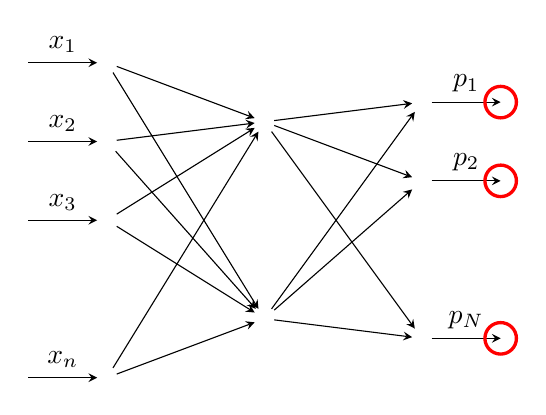
\begin{tikzpicture}[>=stealth]

\foreach \m/\l [count=\y] in {1,2,3,missing,4}
  \node [every neuron/.try, neuron \m/.try] (input-\m) at (0,2.5-\y) {};

\foreach \m [count=\y] in {1,missing,2}
  \node [every neuron/.try, neuron \m/.try ] (hidden-\m) at (2,2-\y*1.25) {};

\foreach \m [count=\y] in {1,2,missing,3}
  \node [every neuron/.try, neuron \m/.try ] (output-\m) at (4,2-\y) {};

\foreach \l [count=\i] in {1,2,3,n}
  \draw [<-] (input-\i) -- ++(-1,0)
    node [above, midway] {$x_\l$};

\foreach \l [count=\i] in {1,n}
  \node [above] at (hidden-\i.north) {};

\foreach \l [count=\i] in {1,2,N}
  \draw [->] (output-\i) -- ++(1,0)
  node [above, midway] {$p_\l$};

\foreach \l [count=\i] in {1,2,N}
  \draw [very thick, color=red] (output-\i)+(1,0) circle (0.2);

\foreach \i in {1,...,4}
  \foreach \j in {1,...,2}
    \draw [->] (input-\i) -- (hidden-\j);

\foreach \i in {1,...,2}
  \foreach \j in {1,...,3}
    \draw [->] (hidden-\i) -- (output-\j);

  \end{tikzpicture}
\end{figure}
\begin{center}
  Some explain the output one-by-one,
\end{center}

        \begin{center}
          But a probability distribution lives on a simplex,\\
          \textbf{The relative information matter!!}
        \end{center}
        
      \end{frame}

  \begin{frame}
  \frametitle{The Shapley values in machine learning}

\tikzset{%
  every neuron/.style={
    circle,
    draw,
    minimum size=0.5cm
  },
  neuron missing/.style={
    draw=none, 
    scale=2,
    text height=0.333cm,
    execute at begin node=\color{black}$\vdots$
  },
}
    
\begin{figure}
  \centering
  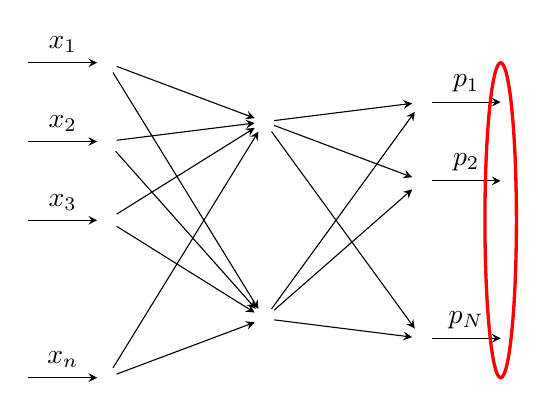
\begin{tikzpicture}[>=stealth]

\foreach \m/\l [count=\y] in {1,2,3,missing,4}
  \node [every neuron/.try, neuron \m/.try] (input-\m) at (0,2.5-\y) {};

\foreach \m [count=\y] in {1,missing,2}
  \node [every neuron/.try, neuron \m/.try ] (hidden-\m) at (2,2-\y*1.25) {};

\foreach \m [count=\y] in {1,2,missing,3}
  \node [every neuron/.try, neuron \m/.try ] (output-\m) at (4,2-\y) {};

\foreach \l [count=\i] in {1,2,3,n}
  \draw [<-] (input-\i) -- ++(-1,0)
    node [above, midway] {$x_\l$};

\foreach \l [count=\i] in {1,n}
  \node [above] at (hidden-\i.north) {};

\foreach \l [count=\i] in {1,2,N}
  \draw [->] (output-\i) -- ++(1,0)
  node [above, midway] {$p_\l$};

\foreach \i in {1,...,4}
  \foreach \j in {1,...,2}
    \draw [->] (input-\i) -- (hidden-\j);

\foreach \i in {1,...,2}
  \foreach \j in {1,...,3}
    \draw [->] (hidden-\i) -- (output-\j);

  \draw [very thick, color=red] (5,-0.5) ellipse (0.2 and 2);
    
  \end{tikzpicture}
\end{figure}
        \begin{center}
          We will explain the probablities all together using the\\
          \emph{Aitchison geometry of the simplex}.
        \end{center}
        
  \end{frame}

\section{Compositional data analysis}

\begin{frame}
\frametitle{Compositional data analysis}

\end{frame}

\section{Shapley composition on the simplex}

\begin{frame}
\frametitle{Shapley composition on the simplex}

\end{frame}

\section{Explaining a prediction with Shapley compositions}

\begin{frame}
\frametitle{Explaining a prediction with Shapley compositions}

\end{frame}

\section{Discussion and conclusion}

\begin{frame}
\frametitle{Discussion and conclusion}

\end{frame}


\begin{frame}[t,allowframebreaks]
   \frametitle{References}
    \printbibliography
  \end{frame}


\begin{frame}
\frametitle{Thank you!!}


\end{frame}



\end{document}
%%% Local Variables:
%%% mode: latex
%%% TeX-master: t
%%% End:
